\subsection{Планарные графы}

\subsubsection{Определение}

\textbf{Планарным} называется неориентированный граф $G$ (множество вершин $V$ и ребёр $E$), который можно нарисовать на плоскости так, чтобы никакие два ребра не пересекались, кроме общих концов. Такое представление называется \emph{планарным вложением} графа.

\subsubsection{Примеры}

\begin{itemize}[leftmargin=*]
  \item Граф $K_4$ (полный граф на четырёх вершинах) является планарным.
  \item Графы $K_5$ и $K_{3,3}$ не являются планарными (теорема Куратовского, см.~ниже).
\end{itemize}

\subsubsubsection*{Планарный пример: $K_4$}

\begin{center}
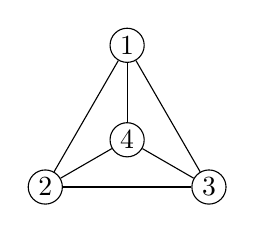
\begin{tikzpicture}[scale=1, every node/.style={circle,draw,inner sep=1.5pt}]
  \node (1) at (90:1.2) {$1$};
  \node (2) at (210:1.2) {$2$};
  \node (3) at (330:1.2) {$3$};
  \node (4) at (0,0) {$4$};
  \foreach \u/\v in {1/2,1/3,1/4,2/3,2/4,3/4}
    \draw (\u) -- (\v);
\end{tikzpicture}

\small Рис. 1. Планарное вложение полного графа $K_4$.
\end{center}

\subsubsubsection*{Непланарный пример: $K_5$}

\begin{center}
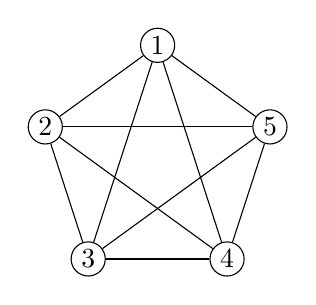
\begin{tikzpicture}[scale=1, every node/.style={circle,draw,inner sep=1.5pt}]
  \node (1) at (90:1.5) {$1$};
  \node (2) at (162:1.5) {$2$};
  \node (3) at (234:1.5) {$3$};
  \node (4) at (306:1.5) {$4$};
  \node (5) at (18:1.5) {$5$};
  \foreach \u/\v in {1/2,1/3,1/4,1/5,2/3,2/4,2/5,3/4,3/5,4/5}
    \draw (\u) -- (\v);
\end{tikzpicture}

\small Рис. 2. Попытка вложения полного графа $K_5$ с неизбежными пересечениями.
\end{center}

\subsubsection{Формула Эйлера}

Для связного планарного графа справедлива \emph{формула Эйлера}:
\[
  V - E + F = 2,
\]
где $V = |V(G)|$ — число вершин, $E = |E(G)|$ — число ребер, а $F$ — число граней (областей плоскости, включая внешнюю).

\paragraph{Пример.} В графе $K_4$ имеем $V=4$, $E=6$. Рассчитаем $F$:
\[
  4 - 6 + F = 2 \;\Longrightarrow\; F = 4.
\]
Действительно, при планарном вложении мы получаем три внутренних треугольника и одну внешнюю область.

\subsubsection{Критерии планарности}

\begin{itemize}[leftmargin=*]
  \item \textbf{Теорема Куратовского:} Граф планарен тогда и только тогда, когда он не содержит подграфа, гомоморфного $K_5$ или $K_{3,3}$.
  \item \textbf{Теорема Вагнера:} Упрощённый критерий: нет миноров $K_5$ и $K_{3,3}$.
\end{itemize}

\subsubsection{Свойства и ограничения}

\begin{enumerate}[label=\arabic*)]
  \item Для простого планарного графа с $V\ge3$ всегда выполняется
  \[
    E \le 3V - 6.
  \]
  Если, кроме того, нет треугольников (циклов длины 3), то
  \[
    E \le 2V - 4.
  \]
  \item Минимальный непланарный граф имеет $V=5$, $E=10$ (граф $K_5$) или $V=6$, $E=9$ (граф $K_{3,3}$).
\end{enumerate}

\subsubsection{Применения}

\begin{itemize}[leftmargin=*]
  \item \emph{Географические карты}: раскраска областей так, чтобы соседние области различались цветом (теорема о четырёх красках).
  \item \emph{Схемотехника}: прокладка дорожек на печатных платах без пересечений.
  \item \emph{Графический дизайн}: автоматическая укладка элементов схем и диаграмм.
\end{itemize}

\subsubsection{Источники}

\begin{itemize}
  \item Д.Б.\,West, \emph{Introduction to Graph Theory}, Prentice Hall.
  \item В.\,Д.\,Мазурин, \emph{Дискретная математика: графы и алгоритмы}.
  \item \href{https://ru.wikipedia.org/wiki/Планарный_граф}{Википедия: Планарный граф}
  \item \href{https://ru.wikipedia.org/wiki/Теорема_Куратовского}{Википедия: Теорема Куратовского}
\end{itemize}